\outline{1}{How to reach the threshold? A trade-off between efficacy and efficiency of motor rehabilitation in chronic stroke}
\chapter{How to reach the threshold? A trade-off between efficacy and efficiency of motor rehabilitation in chronic stroke}
\label{cha:dose}

\section{Abstract}
It is well known in motor learning research that the gains in motor performance depend on the dose of practice, but also that these gains follow diminishing returns: each additional unit of training yields smaller and smaller gains. 
Recent results from the DOSE trial, a single blind, phase I, randomized controlled trial of four doses (0, 15, 30, or 60 hours) of upper extremity therapy during the chronic phase after stroke, showed a robust dose-response relationship for the Motor Activity Log-Quality of Movement (MAL) (Winstein et al., in preparation).  
Here, we test the hypotheses that: 1) increasing the dose of training leads to an increase in the efficacy of training but a decrease in the efficiency of training, and 2) increasing the duration of training will also decrease the efficiency of training. 
We modeled the changes in the MAL during the train-wait-train-wait-train schedule used in the DOSE trial with novel dynamical mixed-effects models that account for individual responses both during and between training bouts. 
With the learning term, we modeled increase in MAL during training.  
With the forgetting term, we modeled the decrease in MAL following training. 
Using dose as input to the model, we estimated the efficiency of training with dose. 
Using time varying learning rates, we estimated the efficiency of training with duration. 
Results confirmed the dose-response relationship previously found. 
The models also showed a decrease of efficiency with dose (the greater the doses, the less the gain per hour) and decrease in efficiency with time (the longer the duration of training, the less the gain per hour). 
In addition, the greater the dose, the more the forgetting following training. 
However, the random learning and forgetting coefficients showed a large between subject variability in both increase and decrease in MAL as a function of dose and time. 
In conclusion, our novel model well accounted for the individual dynamics of motor training post-stroke and exhibited a trade-off between the gains due to training on one hand and the intensity and duration of motor training on the other hand. 


\outline{2}{Introduction}
\section{Introduction}
The foundation of neuro-rehabilitation is that sensorimotor learning determines activity-dependent sensorimotor recovery after stroke (Kitago, 2013; Krakauer, 2006). 
Indeed, a number of studies have reported that UE training improves clinical scores (Cirstea, Mitnitski, Feldman,  Levin, 2003; Kamper, McKenna-Cole, Kahn,  Reinkensmeyer, 2002; Kwakkel, Kollen,  Twisk, 2006; McCrea  Eng, 2005) and improves reaching movements’ speed, smoothness, and range (e.g., (Anton et al., 1996)). 
Clinical trials have shown that motor therapy delivered in the subacute to chronic phase can effectively increase spontaneous use and function of the affected limb for individuals with mild to moderate impairments post-stroke (Wolf et al., 2006) (Lohse, Lang,  Boyd, 2014). 
A recent previous meta-analysis of 30 studies of upper and lower extremity rehabilitation therapy after stroke suggested that large doses of therapy lead to clinically meaningful improvements. 
We recently showed in the DOSE trial (Winstein et al. REF) that a measure of upper extremity use, the MAL-QOM, follows robust dose-response relationships in individuals with chronic stroke (more than 6 months post-stroke). 
Thus, in neuro-rehabilitation, like in motor learning, it appears that the change in motor performance depends on the amount of practice (but see REF). 

However, whereas it is well-established in motor learning that gains in performance follow diminishing returns, that is, each additional unit of training yields smaller and smaller gains, such decrease in efficiency of training in neuro-rehabilitation has yet to be shown. 
Assuming different doses of training per unit of time and different durations of training, such changes in efficiency can be conceptualized in two different ways: On one hand, efficiency can change as a function of the amount, or dose, of training. 
On the other hand, efficiency can change as a function of the duration of training. 
For instance, in a study of intensive arm training post-stroke, we showed previously that most gains were acquired in the first training session, with much smaller gains in a second sessions (Park, Kim, Winstein, Gordon,  Schweighofer, 2016) (REF Park et al.)

Following training, it is unclear whether performance gains are maintained, lost, or even increase following training.
On one hand, motor learning and adaptation research suggests that memories decay following training, and as such, the gains due to therapy could decay. 
In addition, in motor adaptation, the decay is often toward a baseline, so the greater the gains, the more the amplitude of the decay. 
However, in some conditions, the gains can be consolidated, exhibiting little decay. 
For instance, in our previous study of arm training, there was little decay even a month post-training (REF). 
On the other hand, we previously proposed that arm use in daily activities post-stroke, if above a threshold, could act to increase use in a virtuous cycle manner(Hidaka, 2012) (Schweighofer, Han, Wolf, Arbib,  Winstein, 2009) (Hidaka et al. REF; Schweighofer et al. REF ). 
Accordingly, if use is high following therapy, there could be further increase in use. 

Here we addressed these questions in an analysis of all assessments of the MAL in the DOSE trial (REF), in which participants with chronic stroke were randomly assigned to 1 of 4 doses: 0, 15, 30, and 60 hours of upper extremity.
The trial was designed according to a train-wait-train-wait-train schedule, in which training was provided in three weeklong bouts of five consecutive visits each separated by one month. 
Because total of 14 assessments were performed before, during, and following therapy, the DOSE trial provides a rich data set to study the question of dose-efficacy, dose-efficiency, time-efficiency, as well as decay post-training. 
In the field of motor adaptation and learning, one often uses state space models to describe the learning processes with a set of inputs, outputs, and variables related by first-order differential equations (Smith, Ghazizadeh,  Shadmehr, 2006) (Lee, 2009) . 
Unlike regression models, state-space models can describe processes that respond to time-varying inputs or stimuli. 
Here, we use a similar approach to model the dynamics of change in arm and hand use during and following neuro-rehabilitation in the DOSE trial. 
We modeled the changes in the MAL during the train-wait-train-wait-train schedule used in the DOSE trial with novel dynamical mixed-effects models that account for individual responses both during and between training bouts. 
Because, as discussed above, it is unclear whether the phase following training will “decay”, as typically do states in state space models, we use first order dynamical models with learning terms to model increase in MAL during training and with a constant forgetting term, to model the decrease in MAL following training. 
Using constant time-varying input to the model across doses, we test the hypothesis (1) that the efficacy of training increases with dose. 
Using dose as time-varying input to the model, we test the hypothesis (2) that the efficiency of training decreases with dose. 
Using time-varying learning rates, we test the hypothesis (3) that the efficiency of training decreases with duration. 
Using time-varying decay term, we then test the hypothesis (4) that dose-dependent forgetting will plateau in the months post-training. 
Finally, we test the hypotheses that forgetting post-training is dose-dependent (5) and that use can modulate the increase in use post-training (6). 



\outline{2}{Methods}
\section{Methods}

\subsection{The DOSE clinical trial}
The current study is a secondary analysis of data from the DOSE trial; we refer the reader to Winstein et al. REF for methodological details. 
Briefly, the DOSE trial was a single blind, phase I, randomized controlled trial of four doses of upper extremity therapy administered in an outpatient setting.  
Participants with chronic stroke (more than 6 months post-onset) were randomized into four intervention groups that varied in the total dose of therapy (0, 15, 30, or 60 hours).  
Each participants signed an informed consent, and the study was approved by the Institutional Review Board of the University of Southern California.

Detailed inclusion and exclusion criteria are described in Winstein et al. REF. 
Briefly, the relevant criteria to the study are: age greater than 21, scores on the impairment UE Fugl-Meyer motor (UEFM) test at baseline were 19-60 out of 66, cognitive function sufficiently preserved to provide informed consent, and no upper extremity sensory impairment or neglect. 
In addition, participants were randomized into one of four groups within four strata by severity and chronicity.  
Participants were stratified by stroke severity based on their baseline UEFM score.  
Individuals with a score between 41-58 were classified as “mild” and those between 19-40 as “moderate”.  
Participants were further stratified by chronicity such that those with stroke onset 6 months to 1.5 years were classified as “early” and those with stroke onset >1.5 years were classified as “late”. 

The intervention was an individualized arm and hand therapy program based on the principle-based Accelerated Skill Acquisition Program (ASAP), which has been described in detail previously (Winstein et al., 2013; Winstein, Lewthwaite, Blanton, Wolf,  Wishart, 2014; Winstein, Wolf,  Schweighofer, 2015). 
In brief, ASAP includes 1) elements of purposeful and skilled movement execution, including challenging and progressive practice, 2) support for patients’ control or autonomy by choices of specific tasks to be practiced, 3) collaborative problem solving to identify and address movement needs, 4) and encouragement of self-direction in extending practice to community contexts (Winstein et al., 2014). 
Using the train-wait-train-wait-train schedule shown in Figure 1A, training was provided in three weeklong bouts of five consecutive visits each separated by one month. 
The total doses were distributed over the three bouts of training, as shown in Figure 1B. 
Therapy was delivered by three different physical therapists over the duration of the trial, who were trained and standardized in ASAP delivery. 

The primary outcome measures in the DOSE trial were the log transformed mean Wolf Motor Function Test time (WMFT) score, and the Motor Activity Log-Quality of Movement rating (MAL-QOM; henceforth referred as MAL). 
The MAL is a semi-structured interview in which participants are asked to recall and rate the quality of movement (QOM) of the paretic arm for 28 activities of daily living. 
It has been used extensively, including in the EXCITE trial, and has good validity and reliability [24]. 
Because we previously showed that the MAL-QOM showed robust and highly significant dose response (Winstein et al. in preparation), we analyzed its dynamics in the study.

In the DOSE trial, each participant performed 14 clinical assessments, which include the MAL, the WMFT, and an arm reach performance and choice task (the BART, REF). 
Trained and standardized research assistants who were blinded to group assignment performed all assessments. 
Assessments were given with the following schedule (see Figure 1 C): 1) twice to assess baseline values in the month before training; 2) in the morning of the first day of training and 3-days training for each of the three 1-week training bouts, and 3) monthly for 6 months following the last bout of training.  

\begin{figure}
	\centering
	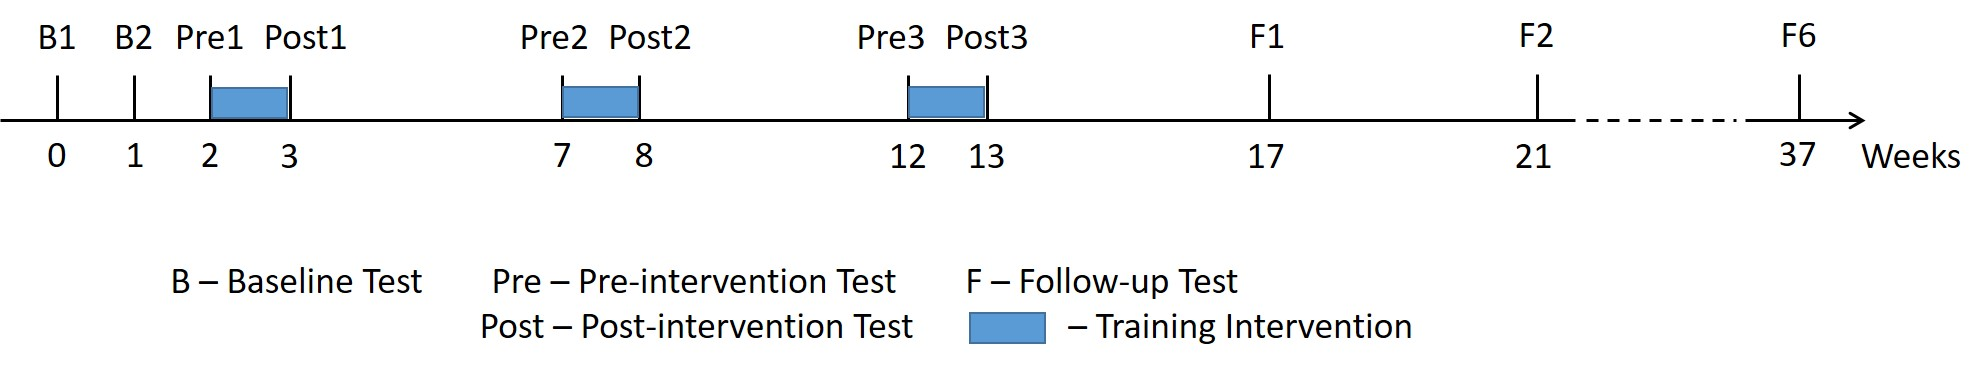
\includegraphics[width=1\linewidth]{figures/dosetimeline}
	\caption[DOSE Study Timeline]{The timeline of DOSE study. Each tick represents a test. Three training intervention periods in between three pairs of pre and post tests.}
	\label{fig:dosetimeline}
\end{figure}


\subsection{Modeling the dynamics of recovery during and after rehabilitation}
\paragraph{Mixed effect dynamical model of MAL}
Our train-wait-train paradigm allow us to study the dynamics MAL during, between, and after training. 
Because of the four different doses, we can compare the dose-efficacy of training, that is, the change in MAL as a function of dose, to the dose-efficiency of training, that is, the change in MAL per hour of training for each dose. 
We can also study possible dose-relationship of forgetting post-training. 
Because of the three separated training bouts, we can compare the duration-efficiency of training, that is, the change in MAL for increasing duration of training, in weeks.  

We modeled the dynamics of MAL with a simple first order linear equation, that was derived from the state space first order dynamics, with two advantages: 1) integration of the dynamics yield a simple, tractable, closed form piece-wise linear solution that can be used in the framework of non-linear mixed effect models (see below) and that can be easily solved with the function nlme in R package nlme (Pinheiro, Bates, DebRoy, Sarkar,  Core Team, 2017), 2) unlike the state-space formulation, which yield decay following training, the model allowed “forgetting” to be either negative or positive. 
In the following, we first discuss the base dynamical model and then the addition of mixed effects to the dynamical model.

In developing dynamical models, we made the following assumptions. 
First, we assumed that training increases the MAL. 
Second, we assumed that following training, the MAL can “spontaneously” change either positively or negatively. 
Thus, be x(t), the MAL at time t, with t in increments of weeks. 
u(t), represents either the timing (test of training efficacy and duration efficiency; Figure 1A) or the dose and timing (test of training efficacy; Figure 1B) of  ASAP training. 
In both cases, u(t) = 0, before, between, and after training bouts (See Figure 1). 
To isolate the effect of training input u(t), we further assume that forgetting is smaller than learning when u(t)≠0. 
Thus, the simplest dynamical model is given by
\begin{equation}\label{fode}
	\frac{dx(t)}{dt} = bu(t) + cv(t)
\end{equation}
where
\begin{equation}
v(t) = 
\begin{cases}
	1, & \text{if}\ u(t) = 0 \\
	0, & \text{otherwise},
\end{cases}
\end{equation}
b and c represent constant “learning” and “forgetting” rates, respectively. 
Here, we note that 1) b will typically be positive but c can be positive or negative; thus “forgetting rate” does not necessarily mean a return to baseline, but a change from post-training and 2) other more complex models can be developed with for instance parameters depending on doses or time (see below). 

The solution to Eqn. (1) is a piece-wise linear equation. 
Thus although the response during each bout and following each bout is linear, the overall solution is non-linear
x=f(x0,b,c,t), where x0 is the MAL at baseline. 
In Supplementary material 1, we show that under certain conditions, state space equation is equivalent to differential equation, and therefore share the same solution, which is a nonlinear function. 
We then use nonlinear mixed effect model to estimate the parameters in this nonlinear solution.

Fitting the model of equation (1) to all subjects would provide a mean response. 
However, the addition of random effects in modeling in rehabilitation is desirable because of the high variability in stroke rehabilitation (Park  Schweighofer, 2017) (REF ).  
Here, we therefore updated the nonlinear function x=f(x0,b,c,t) to include mixed effects. In its general form, the model is given by
\begin{equation}\label{eqn:nonlinear}
	x_i (t)=f(x_{0i},b_i,c_i,t) + \epsilon_i (t)
\end{equation}
where $ x_{0i} $, $ b_i $, $ c_i $ are the mixed effect parameters for individual $ i $ (cite Bates); $ \epsilon_i (t) $ is the residual. 
Below we provide an overview of the main models tested. 
A complete list of models is given in Table 1.

\paragraph{Modeling efficacy and dose-efficiency of training}
\subparagraph{Continuous dose models: } 
To estimate the efficacy of training (the overall effect of training), we let $ u(t)=1 $ during the intervention periods as shown in Fig. \ref{fig:dosefigure2}A. 
To estimate the efficiency of training (the effect of training per hour), we let $ u(t) $ to be the number of treatment hours corresponding to the group, as shown in Fig. \ref{fig:dosefigure2}B.  
To investigate how training efficacy and efficiency depends on dosage of training, the mixed effects of $ b_i $ and $ c_i $ are given by:
\begin{eqnarray}\label{eqn:mixedeffect}
	b_i &=& \beta_1^b + \beta_2^b D_i + \delta_i^b   \nonumber \\
	c_i &=& \beta_1^c + \beta_2^c D_i + \delta_i^c   
\end{eqnarray}
where $ D_i $ is the dosage of training (number of hours per week) that participant $ i $ received, 
$ \beta $ coefficients are fixed effects and the $ \delta_i $ coefficients are random effects. 
To better demonstrate the mixed effect, we also adopt Wilkinson notation to express fixed and random effects. 
For example, the Wilkinson notation for eqn. (3) and (4) is
\begin{eqnarray}
	\text{fixed effect: } b + c  &\sim& \text{dose} \\
	\text{random effect: } b + c &\sim& 1
\end{eqnarray}
Fixed effect parameters are represented by, for example, b.(Intercept) and b.dose.

\subparagraph{Categorical dose models: } 
To study how efficacy and efficiency depends on the four doses, we also developed model in which dosage of training is taken as categorical variable, the formula becomes
\begin{equation}
	b_i = \beta_1^b + \beta_2^b D_{i2} + \beta_3^b D_{i3} + \beta_4^b D_{i4} + \delta_i^b
\end{equation}
Where $ D_{ij} $ is 1 when participant i belongs to group j, 0 otherwise. 
The formula for $ c_i $ is in the same structure.

\subparagraph{Modeling time-efficiency}
To study the effect of training in successive bouts, we further assumed b can take different values during training. 
Here again, we considered both continuous and categorical models of time.

In the models with continuous effect of time, we considered a linear dependence of b (and c) on training period k (k=1,2,3), namely
\begin{equation}\label{eqn:timingcat}
	b(k) = \beta_1^b + \beta_2^b (k-1) + \delta_i^b
\end{equation}
As above, the initial condition was modeled with equation 5.  

In the models with categorical effect of time, we modeled independent values of b and c at different training period, namely
\begin{equation}
	b = \beta_k^b,  k = 1,2,3
\end{equation}

Note that in this parameterization, we only considered fixed effects for b and c.

\subparagraph{Modeling decay post-training}
To study the effects of training on forgetting, we develop two additional models. 
In the first model, we test the hypothesis that decay in the six months post-training is due to both dose and the average MAL in the six months post-training. 
For this, we model 
\begin{equation}
	c_3 = \beta_1^{c_3} + \beta_2^{c_3} + \beta_3^{c_3}\text{MAL}_{\text{av}_i} + \delta_i^{c_3}
\end{equation}
with the prediction that $ \beta_2^{c_3} < 0 $ and $ \beta_3^{c_3} > 0 $.

In the second model, we test whether all subject return to their initial baseline or maintain gains in MAL following training.
For this, we slice the 6 months post-training in three equal slices of 2 months, and define three post-training decay parameters $ c_3 $, $ c_4 $, and $ c_5 $ for each 2 months period. 
For each, we assume a dose relationship such that: 
\begin{equation}
	c_k = \beta_1^{c_k} + \beta_2^{c_k} D_i + \delta_i^{c_k}, k = 3,4,5
\end{equation}

\subparagraph{Model fitting}
Model fits were performed using the nlme() function in R (Pinheiro et al., 2017). 
For categorical models, the 0 dose group was used as the reference group, such that the group effects for the other three dose groups are represented with respect to the 0 group. 
For these models, the R function intervals() was used to construct 95\% confidence intervals on parameters.

In addition, because we previously showed that the initial MAL depends on impairment (Wintein et al. 2017), we tested the effect of initial MAL as 
\begin{equation}
	x_{0i} = β_1^{x_0} + β_2^{x_0} \text{FM}_i + \delta_i^{x_0}
\end{equation}
where $ \text{FM}_i $ is the initial UEFM score of participant $ i $.

For all models, inclusion co-variates and random effects was based on via the log-likelihood ratio test for nested models and, for non-nested models on Bayesian Information Criteria (BIC), which provides a measure of quality of fit by minimizing fitting error and penalizing the number of model parameters. 

We used maximum likelihood to estimate parameters. Additional statistical analyses were performed in R 3.4.0. 
Statistical significance was predetermined at p < 0.05. 

Note on doses included in the model: the nominal doses are 0, 15, 30, and 60 hours of ASAP therapy. 
However, each assessment, in addition to the MAL, comprised reaching tests comprised of 100 of movements (see Kim et al. Submitted) as well as the WMFT test, in which subjects perform arm and hand movements. 
Because these tests lasted for approximately 1 hours, two hours per training bouts were added to the actual dose of training in the model. 
Thus, whereas the actual doses of therapy were 0, 5, 10, and 20 hours per week, the doses used in the model were 2, 7, 12, and 22 hours (See Figure 1B). 
In addition, for taking into account a possible testing effect (highly probable given our previous work showing the repeated arm reach training in the chronic phase can induce long-lasting changes in performance REF), the addition of a non-zero dose for the control group allows to define a learning rate parameter for this dose, and therefore allows us to compare learning rate b in other groups to this reference group.


\outline{2}{Results}
\section{Results}

\subsection{Modeling MAL dynamics}
Results presented in Table 1 show the final models selected for all hypotheses tested as well as the best fitting model. 
In all cases, incorporating the fixed effect of initial UEFM on the initial MAL improved the fit, with significant effect for all model considered (p < 0.01 for all models; because of the consistency of this effect, these coefficients will not be discussed anymore and are not shown in the supplementary tables).

Figure 2A shows both actual data for all subjects and illustration of the fit for the best fitting model 6. 
As can be seen the model fits all subject’s data well: all of the initial conditions, change in MAL during training, and following training are well accounted for. 
In Figure 2B, we showed the model fits re-arranged by nominal doses. 
Note how, larger doses appear to increase response to training, that is the efficacy of training, but also increase forgetting post-training. 
These results, as well as decreased efficacy, will be demonstrated below.

\subsection{Training Efficacy}
The results of fit for the models for testing dose-training efficacy (models 1.1 and 1.2 in Table 1) are shown in Figure 3A and supplementary table 1. 
As suggested by the individual responses of Figure 2A, increasing dose of training increases the efficacy of training, as shown by the positive slope between dose and the increase in MAL per session (parameter b.dose = 0.002; p < 0.01). 
Figure 3A, and inspection of the coefficients of the categorical model show, however, that this dose efficacy is mostly driven by the 60 hour dose (parameter $ b.dose_hour $ 60 is greater than b.(Intercept) parameter p < 0.05).

Whereas increasing dose increases MAL during training, the same continuous dose model show that following training, there is an increase in forgetting for larger doses, as shown by the negative slope between dose and the change in MAL between sessions (parameter c.dose =  negative  -0.0001**; p < 0.05 – Figure 3B). 
Note however, that for 0 dose, c is slightly positive although not significantly different from 0 (c.(Intercept) = 0.001). A model with categorical dose effect on c (results in Figure 3B) shows that the dose effect is mostly linear and significant for 30 and 60 hour doses ($ c.dose_hour30 $  -0.0020477 p <  0.05,  $ c.dose_hour60 $  -0.0027305; p<  0.01)

\subsection{Effect of Dose and Timing on Training Efficiency}
The results of fit for the models for testing dose training efficiency (models 2 in Table 1) are shown in Figure 4A and supplementary table 2. 
As a reminder, in these models, the input u(t) is proportional to the dose – as a result, the learning rate parameter reflects the efficiency of training. 
As predicted, increasing dose of training decreases the efficiency of training, as shown by the negative slope on Figure 4A (parameter b.dose is negative  = -0.0001; p < 0.05). 
Figure 4A, and inspection of the coefficients of the categorical model show, that this effect is mostly driven by the 30 and 60 hour doses (both parameters are greater than b.intercept parameter p<0.05).

Similarly, the efficiency of training decreases with the number of bouts of training (model 3 in table 1; Figure 4B). 
The effect is strong with more than a two-fold reduction in gain for the second and third bout compared to the first bout. 
Interestingly, the b3 coefficients (learning rate for the third bout) is not significantly different from 0 (supplementary table 3). 
Thus, the increase due to the third bout of training is small, even for larger doses. 
Such small effects of later bouts of training can be seen in plots of the individual fitted response with this model (Figure 5), notably for the 60 hour group. 
The first session of training largely increases the MAL. 
However, the second and in particular the third session have reduced effect. 
Similarly, it can be seen that for the 15 hour groups, very few subjects benefit from the additional training. 
Accordingly, the coefficient for the third session is near 0 (Figure 4b, and not significantly different from 0 – Supplementary Table 3).

\subsection{Forgetting following training is fast initially but tampers off within 2 months post-training}
In motor learning research, it is commonly observed that forgetting following training is initially fast and then tampers off. 
Here, using a model in which the forgetting over the six months post-training are estimated over three intervals of 2 months (model 4 in Table 1), we show that following the last session of training, forgetting is initially relatively rapid, but by 2 months post-training, forgetting tampers off, which allow patients to maintain some of the gains due to therapy. 
Accordingly, the forgetting parameter immediately training is significantly negative, but the next two parameters are not different from 0 (c3 = -0.003, p = 0.0069, c4 = 0.002, p = 0.1020, c5 = -0.00, p = 1).

\subsection{Forgetting is modulated by use}
As we saw earlier, the higher the dose of training, the more the forgetting. 
However, as has been suggested in previous work (Schweighofer et al., 2009)(REF), and as seem to be indicated in Figure 4 (in which forgetting is only modeled with random effects), spontaneous use of the affected arm in daily activities may act as “self-training”, and reduce forgetting, or even continues to increase use, in a virtuous cycle. 
Thus, here we test the hypothesis that forgetting in the 6 months following training depends not only on dose but also on the average MAL during these 6 months, with greater MAL leading to less forgetting. 
Figure 6 shows that this in indeed the case; the forgetting coefficient depends monotonically on the average MAL, with a threshold near MAL = 3. 
Above this threshold, the forgetting parameters is positive, that is, MAL keeps increasing in a spontaneous manner, without external training.


\section{Discussion and Conclusion}
A 1997 research agenda that emanated from a workshop focused on facilitating patient learning during medical rehabilitation, proposed that “the effectiveness and efficiency of learning-oriented practices will likely be enhanced by well-formulated investigations grounded in available learning theory and research” ((Fuhrer, 1998) p. 560). 
Here, we believe that, in a combination of a 1) novel dynamical models with mixed effects 2) all, novel rehabilitation design following a wait-train-wait approach,  allowed us to dissociate the effects dose and duration of training on the efficacy and efficiency of neurorehabilitation.

Our findings were made possible by our use of novel statistical models of recovery post-stroke based on dynamical models with mixed effects are novel.
Although never applied to stroke, mixed effects dynamical models have been applied to model the action of drugs on a range of diseases (Cazelles Chau, 1997; Tan  Ye, 2000).  
The dynamical component of the model allowed us to obtain a detailed time course of the changes in the MAL with time in response to discrete bouts of training of different doses. 
The use of the mixed-effects in the nonlinear model is motivated by the high variability in lesion, impairment, and responsiveness to therapy in individuals with stroke REF. 
In a previous reach training study with participants with chronic stroke (REF), we used non-linear mixed effects models to dissociate improvement in performance due to learning from highly variable decrease in performance presumably due to fatigue. 
In future studies that record large amount of neural and clinical data, the number of co-variate may be sufficiently large to capture for most of the variance in the data. 
In the current study, the mixed-effects allowed us to model the between- participant variability that is not captured by the co-variates such as the initial MAL, the initial FM, and the dose. 
The inclusion of the random effects the largely improve the fit however. 
For instance, the fitting error of  “best model” (the Log-likelihood) worsens by 23 \% when only initial random effects are included (that is, when learning and decay rate random effects are removed). 
The model with no random effects does not converge at all. 

Our main findings are that whereas larger doses increase the MAL from pre to post-training, but also increase forgetting post-training and decrease the efficiency of training. 
In previous work, we have shown a strong dose response relationship for the MAL in the DOSE trial when solely considering changes due to the three bouts of training. 
Here, fitting dose-efficacy dynamical models that include all the data, in particular the 1-month wait periods between the train bouts, we show that the “learning rates” of the model with dose-independent inputs. 
Because the learning rates with such inputs represent the gain in MAL for each training bout, the dose versus learning rates plot represent a dose-response curve; this results thus confirm our previous finding of a significant dose response relationship (Figure 3). 
This dose response curve is only true during training however. 
Indeed, results show that there is no differences in response accross doses when the median of the first three MAL tests (before training) are compared the median of the last three (ANOVA, p = XX). 
The main cause for this lack of overall efficacy is the very significant dose relationship in the decay following training (Figure 3B), with many participants in large doses showing reduction in the MAL following training (see Figure 2B). 
In addition, participants in the low doses often show a “spontaneous” increase in the MAL following training – we will discuss this phenomenon below. 
Although it is unclear  what causes this dose-dependent forgetting, it resembles decay in motor adaptation (REF), because 1) it is initially fast in the two first month following training before tempering to zero in the last 4 months (see results) and 2) it is greater following greater gains, as seen with adaptation to larger perturbation. 
Although this may be taken with caution, it is therefore possible that training given in the chronic state post-stroke is similar to motor adaptation, which is defined as return of the system to baseline performance in face of perturbation. 
So here, training can be seen as the perturbation, and upon the discontinuation of training, the system returns to its baseline “chronic” state. 

In contrast to the dose-efficacy of training, using a model with inputs that scale to the dose of training, we have shown a decrease in efficiency of training for greater doses. 
With such inputs, the learning rates represent the changes in MAL for each hour of dosing, and therefore represent the efficiency of training. 
Unlike for dose-efficacy, the dose-efficiency results of Figure 4 A show a clear decrease in efficiency with additional hours of the dose of training. 
Each hour of training in the 60 hour dose group is about two times less effective in increasing the MAL than an hour in the 15 hour dose. 
If we consider the training effect due to the pre- and post-trainig tests of an hour each, the effect of 1 hour of these tests in increasing the MAL is about 3 times more efficient than 1 hour in the 60 hour dose. 

Similar to the decrease in dose-efficiency, we also showed a strong decrease in duration-efficiency: the first bout has greater efficiency than the second, itself greater than the third. 
Such decrease is consistent with the well-known negatively accelerated learning curves in motor learning, where each additional unit of practice yields a smaller gain. 
Examination of Figure 4 shows indeed a non-constant decease in efficiency: the decrease is large initially and plateaus thereafter, with the same average efficiency for 30 and 60 hour doses. 
Thus, the decrease in efficiency in motor training in the chronic phase post-stroke, at least with the ASAP methodology, well matches what is expected from motor training of single skills.

Our results have so far painted a rather bleak view of rehabilitation with two major issues: first, despite a dose-response relationship during training, the gains are lost following training. 
Second, the more the dose and the duration of training, the less the efficiency of training. 
However, the increase of the MAL post-training for a number of participants, and in the 0 dose group in particular, casts hope for developing effective rehabilitation methods. 

Increase in the MAL post-training maybe due to a ‘self-training’ affect. 
A model in which we use the dose and average MAL post-training  as covariate for forgetting post-training (Model X; Table XX)– show  that the change in MAL post-training is positively modulated by the average of the level of MAL post-training. 
Thus, if MAL post-training is high, because it was high initially, or because therapy brought the MAL to a high level, then the MAL keeps increasing following training. 
We previously postulated the existence of a threshold in which arm use in daily activities acts as “self-training” and reinforce performance, which then further reinforce us in a virtuous cycle. 
Here, across doses, figure XX shows that there is threshold for the MAL, around 3.5. 
Above this value, uses continues to increase spontaneously post-training. 
Below this value, uses decreases. 
Accordingly, the goal of rehabilitation is therefore to bring the patient above threshold, such that the gains from rehabilitation can be not only maintained but further increased thanks to the patient (implicit) self-training via daily activities. 

But how can we explain the increase in the MAL in the 0 group even for lower MAL values? A possibility is a learning effect of the MAL itself, but if this effect exists, it is probably small because the increase is not seen in most participants in large dose groups. 
An alternative is that assessment, which contains between 100 to 200 movements (depending on subject choice to use their arm, as our test contained both forced and free choice trials) plus the WMFT test, increases the MAL. 
This increase in MAL due to this test would be stronger in the 0 dose group, and still somewhat present in the 15 hour dose group (see Figure 2), but not in the larger dose group because of the reduced efficiency of training in these groups. 
Thus, in the large dose group, the efficiency of these same tests is reduced, and participants in the 30 hours and 60 hours group show decay post-training on average, (although variability is large and in part explained by arm use post-training - see above). 

Taken together these results support a rehabilitation strategy in which the same amount of training is distributed over months not only to increase the MAL during training, but also to maintain the gains. 
Indeed, one of the most robust results of learning theory is the so-called “spacing effect”, according to which the spacing of presentations strongly increases the retention of learned material compared to massed presentations. 
This phenomenon has been extensively studied in word learning research for more than a century (Ebbinghaus, 1913) – see for a review (Druckman  Bjork, 1991). 
Note that the spacing effect can be extremely robust, as in some cases massed practice yields long-term performance less than one half the level from spaced practice. 
Further, it can be truly long-lasting, as (Bahrick, 1987) found enhanced retention up to 8 years after vocabulary learning with spaced presentation. 

\paragraph{Conclusions: implications for clinical practice}
Although our results need to be confirmed, they point to the need of a change in policy and rehabilitation methods: the intensity of training in the chronic state can be relatively small for each bout, but training should be continuously distributed over a life-time. 
Here, please note that “small” is relative, and we do not believe that the amount of training  given in a single session of clinical practice is sufficient, as patients perform only 32 movements session on average (Lang et al., 2009). 
Our assessments contain between 100 to 200 movements plus the WMFT test. 
In addition, we previously showed (REF Park and Schweighofer), that most gains in reaching movements were achieved with approximately 300 movements. 
Thus, our results suggest that intensive bouts of training of a few hundred movements should be given at regular intervals. 
Delivering such training will probably be well suited via technological devices that can assess and train the movements, such the device we proposed previously (REF han et al. and REF, Park et al.). 


\section{Supplementary Materials}
\subsection{State Space Model to Nonlinear Mixed Effect Model}
In the field of motor perturbation adaptation, state space model is adopted to model learning behavior [cite]. 
In particular, the state of the system $ x_k $ at trial $ k $ follows 
\begin{equation}\label{ssm}
x_{k+1} = Ax_k + Bu_k
\end{equation}
Where $ A $ represents retention, and often takes a value slightly smaller than 1; 
where as B, slightly bigger than 0, represents learning due to input $ u_k $ {often indicating the error in motor perturbation adaptation).
	This formula can be written as a differential equation:
	\begin{equation}
	\frac{\Delta x_k}{\Delta t} = \frac{x_{k+1}-x_k}{\Delta t} = \frac{(A-1)x_k}{\Delta t} + \frac{Bu_k}{\Delta t}
	\end{equation}
	Omit index $ k $ and let $ a = (A-1)/\Delta t $, $ b = B/\Delta t $ and $ \Delta t\rightarrow 0 $, we have
	\begin{equation}\label{oode}
	\frac{dx(t)}{dt} = ax(t)+bu(t)
	\end{equation}
	The solution to this differential equation is in general
	\begin{equation}\label{generalsolution}
	x = x_0e^{at} + b\int_0^t e^{a(t-\tau)}u(\tau)d\tau
	\end{equation}
	If $ a $ is small comparing to the time scale concerned (that is to say $ |at_{\text{max}}| \ll 1 $) and $ b $ is comparibly small to $ a $ (that is to say $ \text{lim}\frac{bu_\text{max}}{ax_\text{max}} \leqslant \text{const.} $), then the first order approximation to this solution is
	\begin{equation}\label{specialsolution}
	x = x_0 + x_0at + b \int_0^t u(\tau)d\tau
	\end{equation}
	Let $ c=x_0 a $, the original differential equation \ref{oode} becomes
	\begin{equation}
	\frac{dx(t)}{dt} = bu(t) + c
	\end{equation}
	To isolate the effect of training input $ u(t) $, we further assume that c can be ignored when $ u(t) \neq 0 $, i.e.
	\begin{equation}\label{fode}
	\frac{dx(t)}{dt} = bu(t) + cv(t)
	\end{equation}
	where
	\begin{equation}
	v(t) = 
	\begin{cases}
	1, & \text{if}\ u(t) = 0 \\
	0, & \text{otherwise}
	\end{cases}
	\end{equation}
	Or, in logical notation, $ v(t) = \sim u(t) $. 
	This assumption would be further justified later when we show $ bu(t) $ is much larger than $ c $.
	
	Denote the solution to Eqn. \ref{fode} as nonlinear function $ x=f(x_0,b,c,t) $, we estimate the mixed effect model as
	\begin{equation}\label{eqn:nonlinear}
	x_i (t)=f(x_{0i},b_i,c_i,t) + \epsilon_i (t)
	\end{equation}
	where $ x_{0i} $, $ b_i $, $ c_i $ are the mixed effect parameters which can vary from individual to individual (cite Bates).
	$ \epsilon_i (t) $ is the residual. 
	We choose different mixed effects on $ b_i $ and $ c_i $ to investigate different aspects of training mentioned above.
	
	\textbf{Training Efficacy and Efficiency.}
	To estimate the efficacy of training (the overall effect of training), we let $ u(t)=1 $ during the intervention periods as shown in Fig. \ref{fig:dosefigure2}A. 
	To estimate the efficiency of training (the effect of training per hour), we let $ u(t) $ to be the number of treatment hours corresponding to the group, as shown in Fig. \ref{fig:dosefigure2}B. 
	
	\begin{figure}
		\centering
		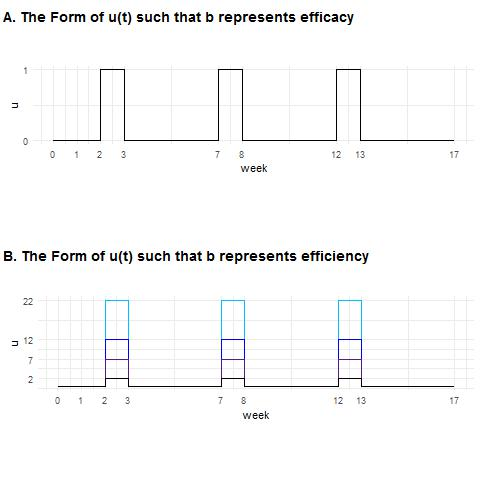
\includegraphics[width=0.7\linewidth]{figures/dosefigure2}
		\caption[Efficacy and Efficiency]{Different training input $u(t)$ for estimating Efficacy and Efficiency. In Panel A, $u(t)$ is either 1 or 0. In Panel B, $u(t)$ is the number of hours received in that training period. $u(t)$ is different for different groups.}
		\label{fig:dosefigure2}
	\end{figure}
	
	To investigate how training efficacy and efficiency depends on dosage of training, we use a linear formula for the mixed effects of $ b_i $ and $ c_i $:
	\begin{eqnarray}\label{eqn:mixedeffect}
	b_i &=& \beta_1^b + \beta_2^b D_i + \delta_i^b   \nonumber \\
	c_i &=& \beta_1^c + \beta_2^c D_i + \delta_i^c   \\
	x_{0i} &=& \beta_1^{x_0} + \beta_2^{x_0} A_i + \delta_i^{x_0} \nonumber
	\end{eqnarray}
	where $ D_i $ is the dosage of training (number of hours per week) participant $ i $ received, 
	$ A_i $ is certain clinical assessment before the training, e.g the initial FM score and/or CST of participant $ i $, 
	$ \beta $ are fixed effects and $ \delta_i $ are random effects. 
	Indexes on the shoulder indicates the parameter to which this fixed or random effect belongs.
	
	In the case when we take the dosage of training as categorical variable, i.e. how efficacy and efficiency depends on the four groups, the formula becomes
	\begin{equation}
	b_i = \beta_1^b + \beta_2^b D_{i2} + \beta_3^b D_{i3} + \beta_4^b D_{i4} + \delta_i^b
	\end{equation}
	Where $ D_{ij} $ is 1 when participant i belongs to group j, 0 otherwise. The formula for $ c_i $ is in the same structure.
	
	\textbf{The Timing of Training}
	To look at the effect of training at different period, we further assume $ b $ and $ c $ can take different values at different intervention periods. 
	We applied this assumption in two ways: 1) A linear dependence of $ b $ (and $ c $) on training period $ k (k=1,2,3) $, namely
	\begin{eqnarray}\label{eqn:timingcat}
	b(k) &=& b_0 + b_t (k-1) \nonumber  \\
	c(k) &=& c_0 + c_t (k-1)
	\end{eqnarray}
	So that we have two more parameters than Eqn. \ref{fode}. 
	
	Due to insufficient data points (too few data points at each training period), we simplify the mixed effects of $ b(k) $ and $ c(k) $:
	\begin{eqnarray}
	b_0 &=& \beta_1^b + \delta_i^b \\
	b_t &=& \beta_2^b
	\end{eqnarray}
	The formula for $ c_0 $ and $ c_t $ is in the same structure.
	
	2) Independent values of $ b $ and $ c $ at different training period, namely
	\begin{equation}
	b = b_k, c = c_k, k = 1,2,3
	\end{equation}
	So that we have four more parameters than Eqn. \ref{fode}. 
	
	We use maximum likelihood to estimate parameters.

